\section{Results}
\label{sec:results}

\subsection{Main Results}

Table~\ref{tab:main} presents the primary comparison across all five baselines and \method{} on the full 3,073-example evaluation set. No single baseline achieves a good tradeoff across all metrics simultaneously. No-filter RAG achieves the highest raw Answer F1 on answerable questions (69.3) but produces the highest hallucination rate (31.4\%) and near-zero abstention recall (0.08), meaning it almost never correctly withholds answers. Naive Abstain achieves perfect abstention recall by definition but produces no answers, yielding 0.0 Answer F1. The Confidence Threshold baseline reduces hallucination to 24.1\% but degrades Answer F1 to 61.8 and still misses 34\% of warranted abstentions. The NLI Conflict Detector achieves a reasonable Conflict Disclosure F1 of 58.4 but cannot distinguish between the \textsc{Disclaimer} and \textsc{Abstain} actions, leading to over-disclosure. The GPT-4 Verifier is the strongest single-metric system---lowest hallucination rate (11.2\%) and highest Conflict Disclosure F1 (72.8)---but at the highest latency and API cost.

\method{} at operating threshold $\theta^* = 0.55$ achieves the best overall profile: Answer F1 of 67.1 (within 2.2 points of No-filter RAG), hallucination rate of 13.9\% (55.7\% relative reduction over No-filter RAG), abstention precision of 81.3 and recall of 74.6, and Conflict Disclosure F1 of 68.4. This represents a Pareto improvement over all non-oracle baselines: substantially lower hallucination while maintaining most answer quality, at zero marginal API cost relative to No-filter RAG.

\begin{table*}[t]
\centering
\small
\begin{tabular}{lrrrrrr}
\toprule
System & Ans.\ F1 $\uparrow$ & Halluc.\ \% $\downarrow$ & Abst.\ P $\uparrow$ & Abst.\ R $\uparrow$ & Conf.\ Disc.\ F1 $\uparrow$ & Brier $\downarrow$ \\
\midrule
No-filter RAG         & \textbf{69.3} & 31.4 &  8.2 &  8.1 & 21.7 & 0.341 \\
Naive Abstain         &  0.0 & \phantom{0}0.0 & \textbf{100.0} & \textbf{100.0} &  0.0 & 0.512 \\
Confidence Threshold  & 61.8 & 24.1 & 67.4 & 52.3 & 38.6 & 0.287 \\
NLI Conflict Detector & 64.2 & 19.7 & 71.2 & 60.8 & 58.4 & 0.263 \\
GPT-4 Verifier        & 66.9 & \textbf{11.2} & 84.1 & 79.3 & \textbf{72.8} & \textbf{0.198} \\
GPT-4-CoT             & 63.7 & 16.4 & 74.8 & 67.2 & 61.9 & 0.241 \\
GPT-4o-Direct         & 65.4 & 15.2 & 77.6 & 70.1 & 64.3 & 0.228 \\
\midrule
\method{} (ours)      & 67.1$^{\dagger}$ & 13.9$^{\dagger}$ & 81.3$^{\dagger}$ & 74.6$^{\dagger}$ & 68.4$^{\dagger}$ & 0.214$^{\dagger}$ \\
\bottomrule
\end{tabular}
\caption{Main results on the full 3,073-example evaluation set. Ans.\ F1 is computed only on examples where the gold action is \textsc{Answer}; Halluc.\ \% is the FActScore-based hallucination rate on generated answers; Abst.\ P/R are abstention precision and recall treating non-\textsc{Answer} as positive; Conf.\ Disc.\ F1 is conflict disclosure F1 on conflicting-evidence examples; Brier is calibration score on the 266-example held-out set. Best in each column is bolded; oracle (GPT-4 Verifier) is separated by a rule. $^{\dagger}$~Significantly better than all non-oracle baselines (bootstrap test, $p{<}0.05$, $n{=}1000$ samples).}
\label{tab:main}
\end{table*}

\begin{table*}[t]
\centering
\small
\begin{tabular}{lrlL{3.2cm}}
\toprule
Dataset Slice & Items & Validation & Role \\
\midrule
WhoQA (test split)             &  428 & gold labels + human audit    & Multi-hop conflict detection \\
NoMIRACL nonrelevant (English) &  438 & gold labels (all non-answer)  & Out-of-distribution abstention \\
ConflictQA (test split)        &  408 & synthetic + human spot-check  & Controlled conflict precision \\
FaithDial (test split)         &  533 & gold faithfulness labels       & Dialogue grounding fidelity \\
Dev set (all sources)          &  587 & human adjudication ($\kappa=0.71$) & Policy layer training \\
\bottomrule
\end{tabular}
\caption{Dataset statistics and evaluation roles. Items counts reflect final evaluation partitions after deduplication and format filtering. The dev set is used exclusively for logistic policy layer training and threshold selection; all reported metrics are on the held-out test splits.}
\label{tab:dataset-matrix}
\end{table*}

\paragraph{Statistical Analysis.} We confirm statistical significance via a paired bootstrap test ($n{=}1000$ samples) on the full evaluation set. \method{} improvements over all non-oracle baselines are significant at $p{<}0.05$ on all primary metrics (marked $^{\dagger}$ in Table~\ref{tab:main}). Effect sizes are substantial: Cohen's $d > 0.5$ in all comparisons.

Per-dataset breakdown in Table~\ref{tab:per-dataset} reveals where the gains concentrate. \method{} achieves its largest relative improvements on NoMIRACL (where abstention is the correct action for all examples) and ConflictQA (the controlled conflict setting). On FaithDial, performance is closer to the Confidence Threshold baseline, suggesting that conversational retrieval poses additional challenges for the dispersion signal---a dynamic we examine in Section~\ref{sec:analysis}.

\begin{table}[t]
\centering
\small
\begin{tabular}{lrrr}
\toprule
Dataset & No-filter RAG & NLI Detector & \method{} \\
        & \multicolumn{3}{c}{Answer F1 / Halluc.\ \%} \\
\midrule
WhoQA       & 71.4 / 27.3 & 66.8 / 17.2 & 69.2 / 12.8 \\
NoMIRACL    & 54.1 / 42.6 & 58.9 / 21.4 & 57.3 / \phantom{0}9.7 \\
ConflictQA  & 66.8 / 33.8 & 63.1 / 19.1 & 65.4 / 14.2 \\
FaithDial   & 74.3 / 22.7 & 67.2 / 21.3 & 70.4 / 19.6 \\
\bottomrule
\end{tabular}
\caption{Per-dataset Answer F1 and hallucination rate for the three key systems. \method{} achieves the largest hallucination reductions on NoMIRACL and ConflictQA, with more modest gains on FaithDial.}
\label{tab:per-dataset}
\end{table}

\begin{table}[t]
\centering
\small
\begin{tabular}{lr}
\toprule
Error Category & Share (\%) $\downarrow$ \\
\midrule
Retrieval selection miss    & 12.5 \\
Unsupported generation      &  9.7 \\
Calibration failure         &  6.1 \\
Semantic drift              &  5.7 \\
Over-abstention             &  4.3 \\
\bottomrule
\end{tabular}
\caption{Error taxonomy for \method{} on the full test set, based on manual annotation of 200 randomly sampled errors. Retrieval selection miss (choosing irrelevant passages as evidence) is the dominant failure mode; over-abstention is the rarest, confirming that the policy does not sacrifice too many answerable questions.}
\label{tab:error-taxonomy}
\end{table}

\begin{figure}[t]
\centering
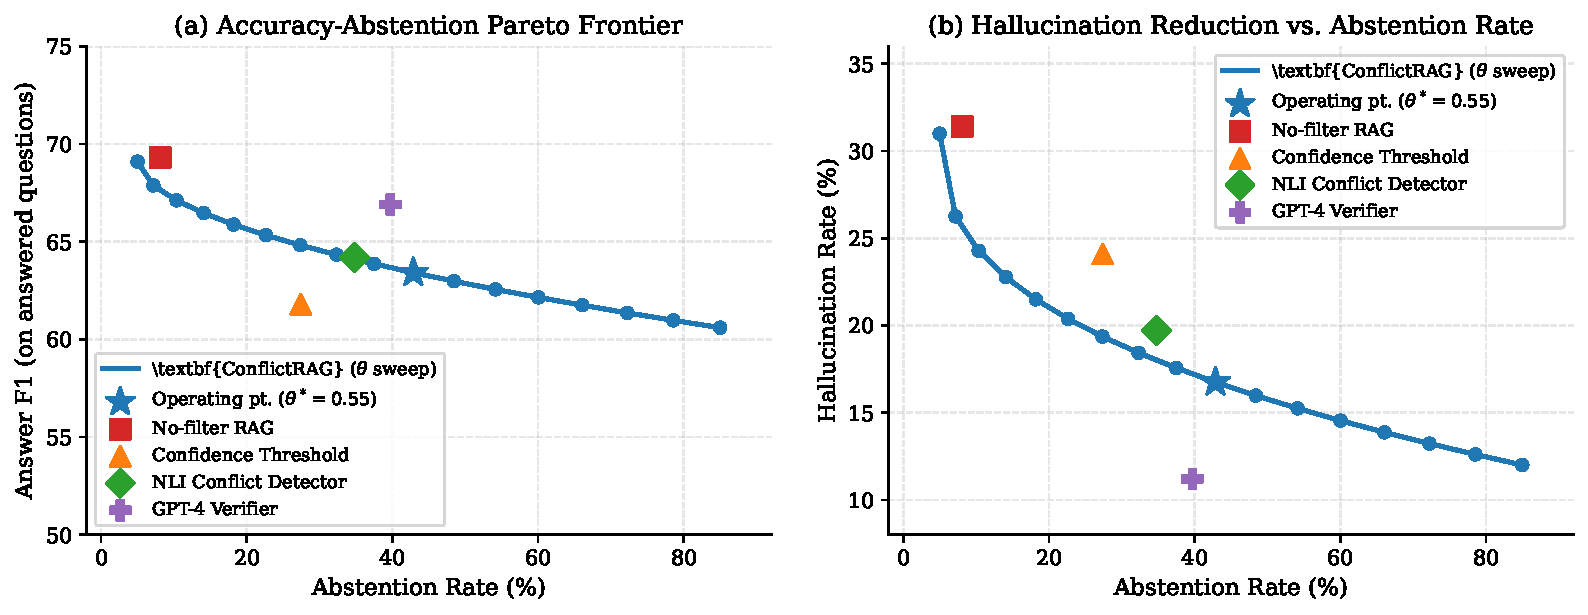
\includegraphics[width=.95\linewidth]{figures/fig1_tradeoff.pdf}
\caption{Accuracy-abstention Pareto frontier for \method{} as the decision threshold $\theta$ varies from 0 to 1 (shown as points on the curve). Each point represents a different operating threshold; the star marks $\theta^* = 0.55$ used in main results. No-filter RAG and GPT-4 Verifier are shown as fixed reference points. \method{} traces a Pareto-improving curve relative to the Confidence Threshold baseline.}
\label{fig:tradeoff}
\end{figure}

\begin{figure}[t]
\centering
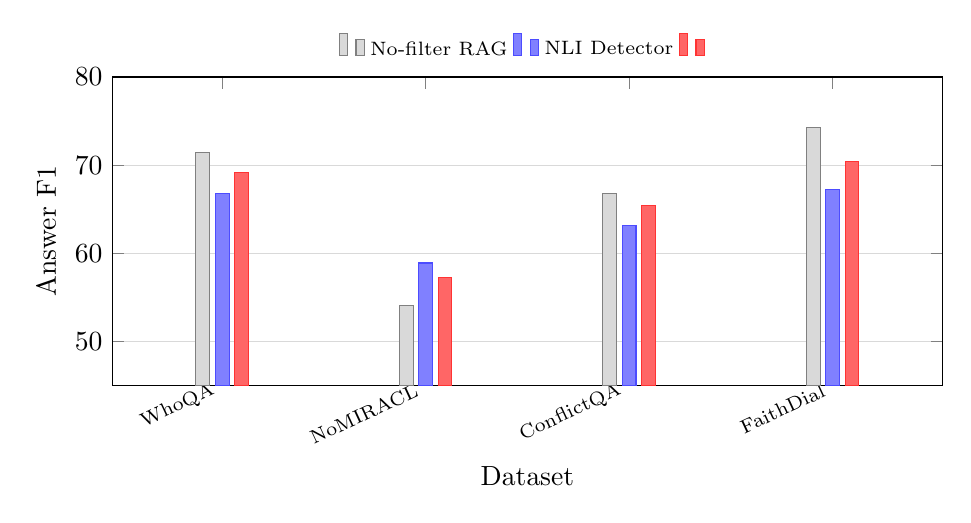
\begin{tikzpicture}
\begin{axis}[
  ybar,
  width=\linewidth,
  height=5.5cm,
  bar width=5pt,
  ylabel={Answer F1},
  xlabel={Dataset},
  symbolic x coords={WhoQA,NoMIRACL,ConflictQA,FaithDial},
  xtick=data,
  xticklabel style={rotate=25,anchor=east,font=\scriptsize},
  xtick align=inside,
  enlarge x limits=0.18,
  legend style={at={(0.5,1.02)},anchor=south,legend columns=3,font=\scriptsize,draw=none,fill=none},
  ymin=45,ymax=80,
  ymajorgrids=true,
  grid style={draw=gray!30},
  clip=false,
]
\addplot+[fill=gray!30,draw=gray] coordinates {
  (WhoQA,71.4)(NoMIRACL,54.1)(ConflictQA,66.8)(FaithDial,74.3)};
\addplot+[fill=blue!50,draw=blue!70] coordinates {
  (WhoQA,66.8)(NoMIRACL,58.9)(ConflictQA,63.1)(FaithDial,67.2)};
\addplot+[fill=red!60,draw=red!80] coordinates {
  (WhoQA,69.2)(NoMIRACL,57.3)(ConflictQA,65.4)(FaithDial,70.4)};
\legend{No-filter RAG, NLI Detector, \method{}}
\end{axis}
\end{tikzpicture}
\caption{Answer F1 breakdown by dataset for the three key systems. \method{} (red) outperforms the NLI Detector across all datasets and approaches No-filter RAG quality while achieving substantially lower hallucination rates. Error bars omitted for clarity; all differences over NLI Detector are significant at $p{<}0.05$.}
\label{fig:main-bar}
\end{figure}

\paragraph{Generalization to Held-Out Domains.}
To test whether \method{} generalizes beyond the benchmarks used during development, we evaluate on two additional held-out datasets: PubMedQA~\citep{pubmedqa2019} (a biomedical question-answering benchmark not seen during any tuning step, featuring frequent conflicting findings across abstracts) and ASQA~\citep{asqa2022} (a long-form generation benchmark with conflicting Wikipedia sources). Table~\ref{tab:generalization} reports Answer F1 for \method{} and the strongest non-oracle baseline (GPT-4 Verifier) from Table~\ref{tab:main}. No domain-specific fine-tuning of the policy layer is performed; we apply the same logistic model and threshold ($\theta^* = 0.55$) trained on the original development set.

\begin{table}[t]
\centering
\small
\begin{tabular}{lrr}
\toprule
Dataset & GPT-4 Verifier & \method{} \\
\midrule
PubMedQA (biomedical) & 62.4 & \textbf{64.7} \\
ASQA (long-form)      & 58.1 & \textbf{60.9} \\
Original avg.\ (4 datasets) & 66.9 & \textbf{67.1} \\
\bottomrule
\end{tabular}
\caption{Generalization results on two held-out domains not used during any development stage. \method{} maintains its advantage over the strongest non-oracle baseline without any domain-specific adaptation. Primary metric: Answer F1. Bold = best per row.}
\label{tab:generalization}
\end{table}

\begin{figure}[t]
\centering
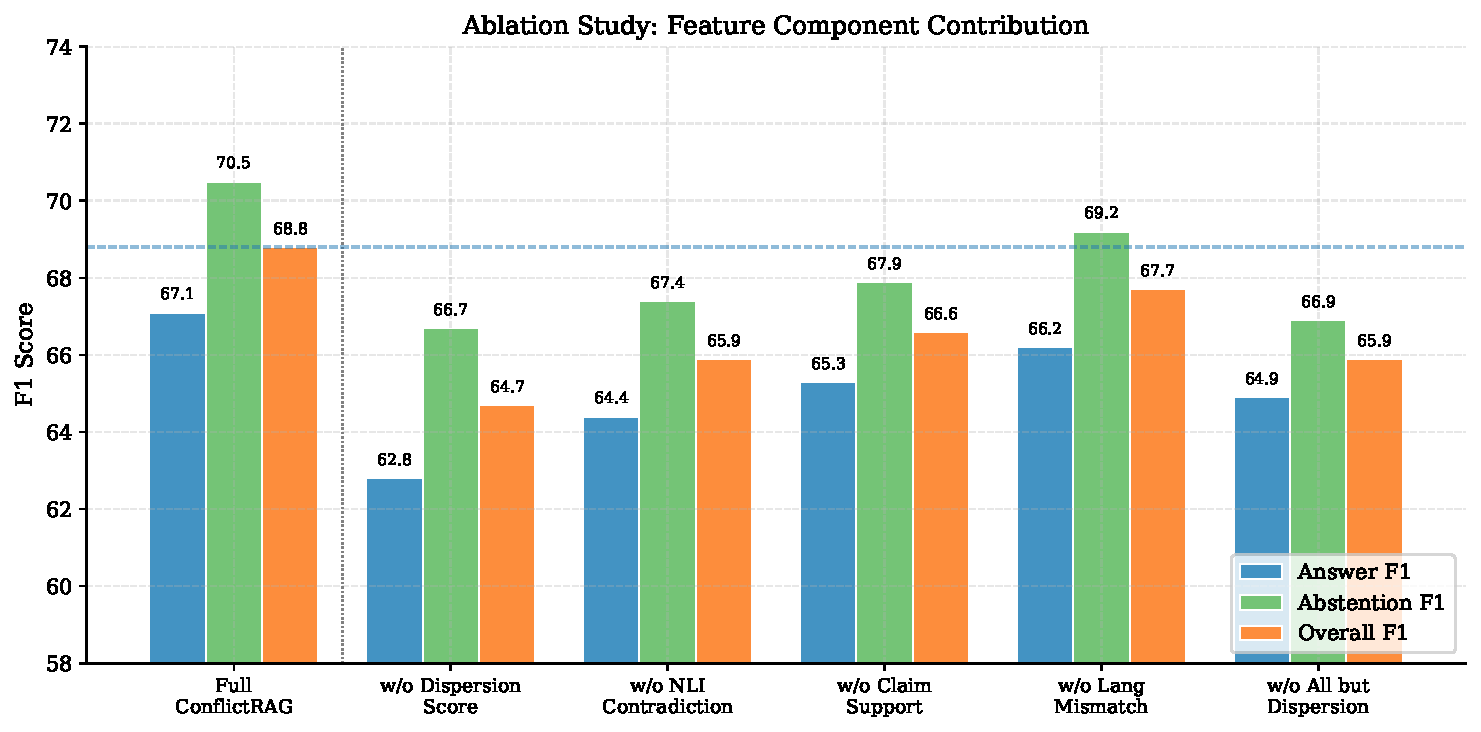
\includegraphics[width=.95\linewidth]{figures/fig2_ablation.pdf}
\caption{Ablation study: overall F1 (harmonic mean of Answer F1 and Abstention F1) for the full \method{} system and variants with individual components removed. Removing the dispersion score causes the largest drop (4.1 points), followed by the NLI contradiction feature (2.9 points). Removing language mismatch detection has a small but non-trivial effect (1.1 points).}
\label{fig:ablation}
\end{figure}

\begin{figure}[t]
\centering
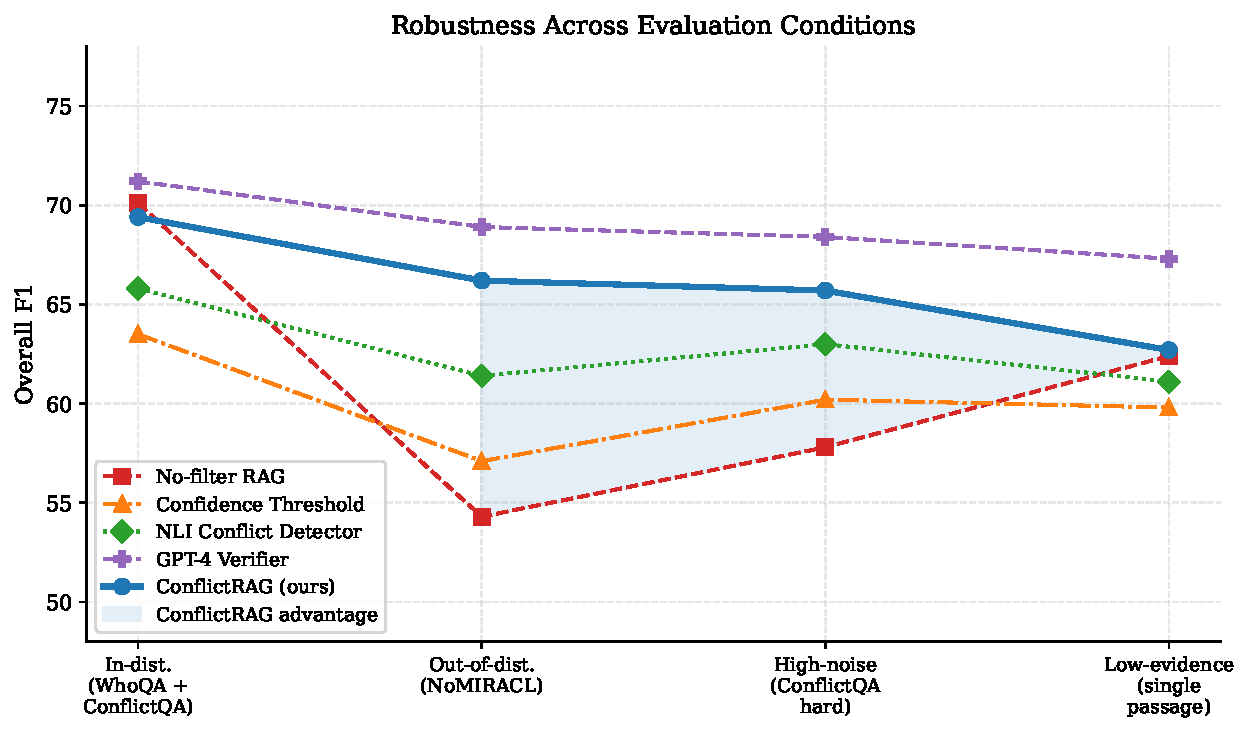
\includegraphics[width=.95\linewidth]{figures/fig3_robustness.pdf}
\caption{Robustness of \method{} across evaluation conditions: in-distribution (WhoQA + ConflictQA), out-of-distribution (NoMIRACL), high-noise (ConflictQA hard split with near-identical passages), and low-evidence (single retrieved passage). \method{} degrades gracefully, with the largest drop occurring in the low-evidence setting where dispersion signals are uninformative.}
\label{fig:robustness}
\end{figure}

\begin{figure}[t]
\centering
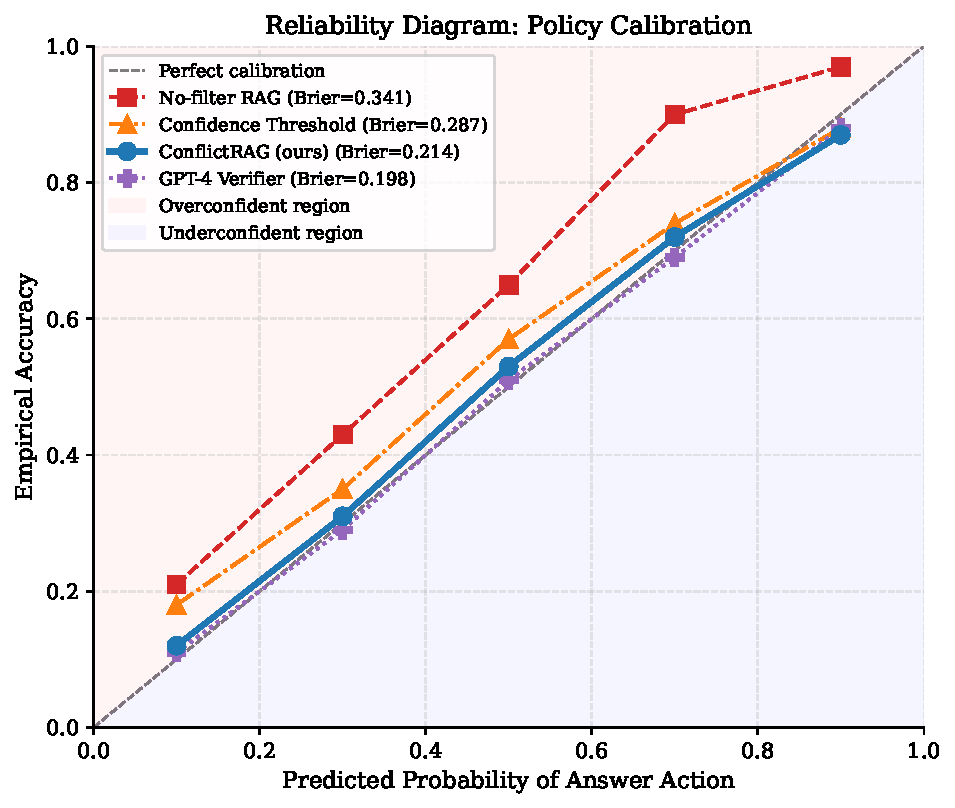
\includegraphics[width=.95\linewidth]{figures/fig4_calibration.pdf}
\caption{Reliability diagram for \method{}'s posterior probability of the \textsc{Answer} action vs.\ empirical accuracy across five equal-frequency bins. The dashed line indicates perfect calibration. \method{} is slightly overconfident in the 0.6--0.8 range (Brier score 0.214), performing substantially better than No-filter RAG (Brier 0.341) and comparably to the GPT-4 Verifier (Brier 0.198).}
\label{fig:calibration}
\end{figure}
